%!TEX root = HW2.tex
\section{15 Cities}
\subsection{Results}
For 15 cities, the algorithms all perform decently well.  The evolutionary algorithm was able to find the best solution.  SA and MCTS are both able to find near optimal algorithms.  EA takes significantly longer than the other two algorithms.  Additionally, SA has the largest variance of each iteration of all the methods between runs while EA and MCTS have similar amounts of variance in each iteration during the search process.    

One reason for EA's better performance is that it holds many more solutions in memory at a time and can compare them against each other.  The other methods hold only one or two solutions at a time and make comparisons based on those two only.  In this implementation of EA, the best solution can never be removed.  If an optimal solution is discovered, it will not be discarded which is true for MCTS, but not SA.  In all cases, EA decreases in distance the quickest.  This may be due to having acces to many solutions that it can quickly hone in on a promising solution.  Although, this may be problematic later on if this is a local minimum.

SA may struggle to get to the optimal solution if it is currently at a state that is near the optimal solution.  If more than a single switch of two consecutive states is requried to achieve a solution, then SA is unlikely to get to that solution.

MCTS has to hold a tree structure which can get quite large in memory.  Each iteration can add a new node to the tree and requires several calculations to update the tree with every iteration.  

% Put table with run time and solution quality results
\begin{table}[H]
\centering
\label{my-label}
\begin{tabular}{|c|c|c|c|c|c|}
\hline
Algorithm               & \begin{tabular}[c]{@{}c@{}}Total Solutions\\ Generated\end{tabular} & \begin{tabular}[c]{@{}c@{}}Average Min\\ Distance\end{tabular} & St Dev & \begin{tabular}[c]{@{}c@{}}Average\\ Run Time (s)\end{tabular} & St Dev \\ \hline
Simulated Annealing     & 10,000                                                              & 7,685                                                          & 994     & 4.72e-6                                                    & 3.8e-6 \\ \hline
Evolutionary Algorithm  & 10,000                                                              & 5,861                                                          & 359    & 4.39                                                       & 0.17   \\ \hline
Monte Carlo Tree Search & 10,000                                                              & 5,916                                                          & 289    & 2.19                                                       & 0.08   \\ \hline
\end{tabular}
\caption{Comparison of Solution Quality and Run Time for Each Method with 15 Cities}
\label{tab:15Comparison}
\end{table}


% insert image of example solutions found by search

\begin{figure}[H]
	\centering
    \begin{minipage}{0.45\textwidth}
        \centering
        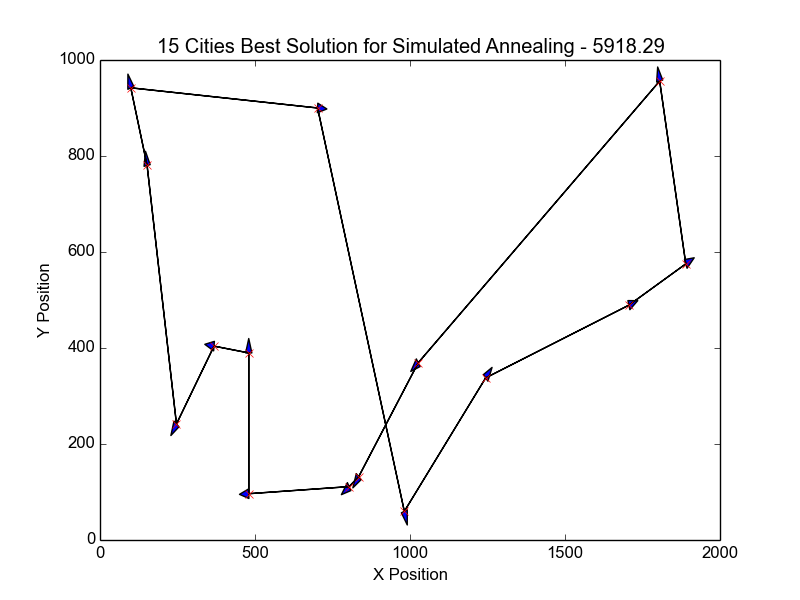
\includegraphics[width=0.9\textwidth]{15City_SA.png} % second figure itself
        \caption{Best Solution for 15 Cities with Simulated Annealing}
        \label{fig:15city_SA}
    \end{minipage}\hfill
    \begin{minipage}{0.45\textwidth}
        \centering
        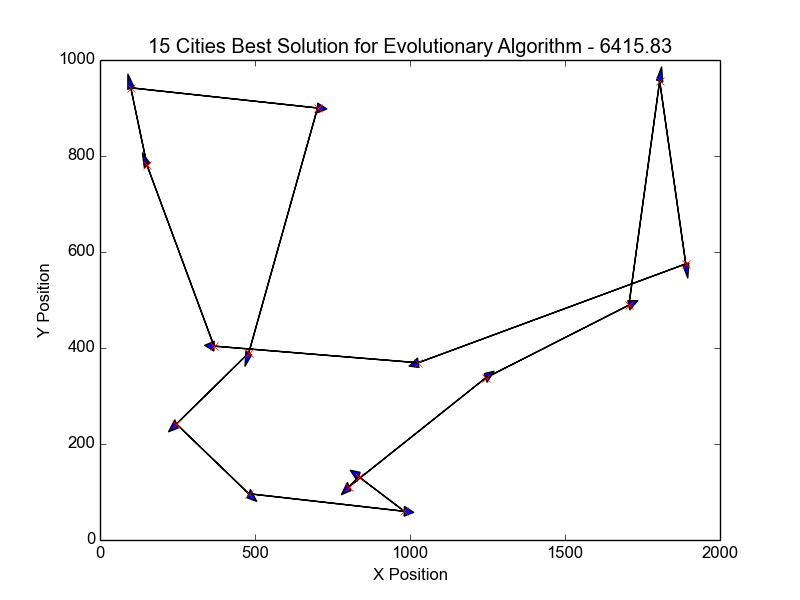
\includegraphics[width=0.9\textwidth]{15City_EA.png} % first figure itself
        \caption{Best Solution for 15 Cities with Evolutionary Algorithm}
        \label{fig:15city_EA}
    \end{minipage}\hfill
    \begin{minipage}{0.45\textwidth}
        \centering
        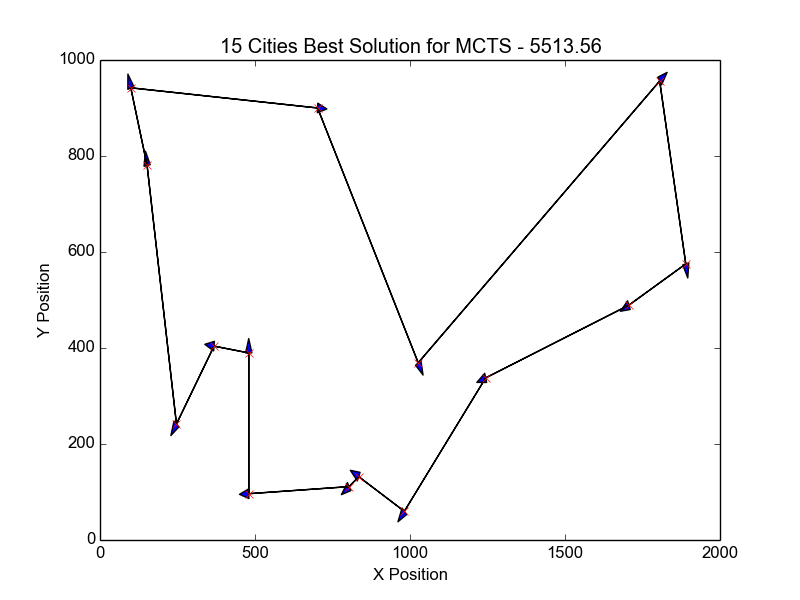
\includegraphics[width=0.9\textwidth]{15City_MCTS.png} % third figure itself
        \caption{Best Solution for 15 Cities with MCTS}
        \label{fig:15city_MCTS}
    \end{minipage}\hfill
    \begin{minipage}{0.45\textwidth}
		\centering
		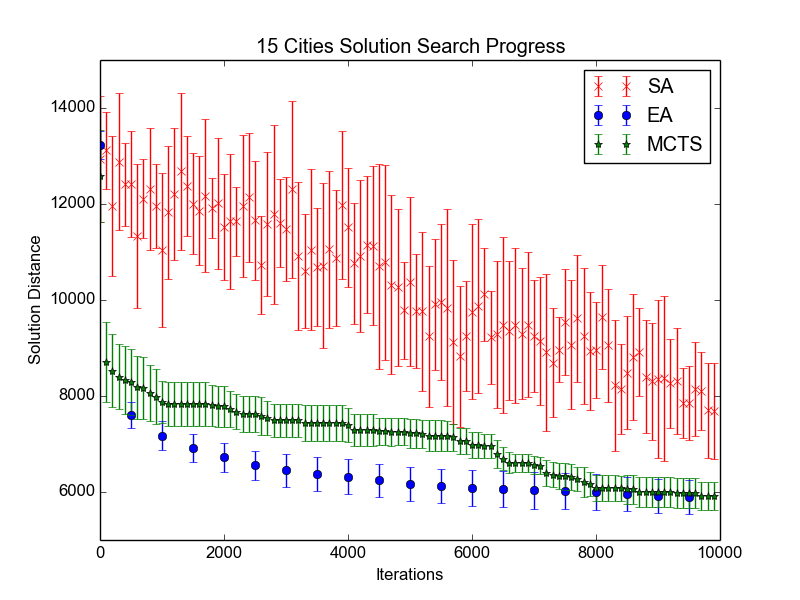
\includegraphics[width=0.9\textwidth]{15City_Solutions.png}
		\caption{Solution Progression for 15 Cities}
		\label{fig:15city_Solution}
    \end{minipage}\hfill
\end{figure}
